%%%%%%%%%%%%%%%%%%%%%%%%%%%%%%%%%%%%%%%%%%%%%%%%%%%%%%%%%%%%%%%%%%%%%%%%%%%%%%%%%%%%
% Do not alter this block (unless you're familiar with LaTeX
\documentclass{article}
\usepackage[margin=1in]{geometry} 
\usepackage{amsmath,amsthm,amssymb,amsfonts, fancyhdr, color, comment, graphicx, environ}
\usepackage{tikz}
\usepackage{algorithm}
\usepackage{algpseudocode}
\usepackage{xcolor}
\usepackage{mdframed}
\usepackage[shortlabels]{enumitem}
\usepackage{indentfirst}
\usepackage{hyperref}
\hypersetup{
    colorlinks=true,
    linkcolor=blue,
    filecolor=magenta,      
    urlcolor=blue,
}


\pagestyle{fancy}


\newenvironment{problem}[2][Problem]
    { \begin{mdframed}[backgroundcolor=gray!20] \textbf{#1 #2} \\}
    {  \end{mdframed}}

% Define solution environment
\newenvironment{solution}
    {\textit{Proof:}}
    {}

\renewcommand{\qed}{\quad\qedsymbol}

% prevent line break in inline mode
\binoppenalty=\maxdimen
\relpenalty=\maxdimen

\newtheorem{theorem}{Theorema}[section]
\newtheorem{lemma}[theorem]{Lemma}
\newtheorem{corollary}{Corollarium}[section]
\newtheorem{proposition}{Propositio}[theorem]
\theoremstyle{definition}
\newtheorem{definition}{Definitio}[section]

\theoremstyle{definition}
\newtheorem{axiom}{Axioma}[section]

\theoremstyle{remark}
\newtheorem{remark}{Observatio}[section]
\newtheorem{hypothesis}{Coniectura}[section]
\newtheorem{example}{Exampli Gratia}[section]


%%%%%%%%%%%%%%%%%%%%%%%%%%%%%%%%%%%%%%%%%%%%%
%Fill in the appropriate information below
\lhead{Your name: Harry Han}
\rhead{CGT Fall 2023} 


%%%%%%%%%%%%%%%%%%%%%%%%%%%%%%%%%%%%%%%%%%%%%

\begin{document}
\begin{centering}\textbf{Assignment 2: Due Friday 27 October 15:00, via Gradescope on Learn}\end{centering}

\begin{problem}{1} (5pts)

Show that if $G$ is 2-connected and the degree of every vertex is at least three, then there exists some edge $e$ such that $G - e$ is still 2-connected.

\begin{itemize}
\item \textbf{\underline{Remark:} the book doesn't say it explicitly, but a $k$-connected graph is assumed to have more than $k$ vertices. }

\item \textbf{\underline{Fact 1}, which you can use without proving: a graph $G$ is 2-connected if and only if any two \underline{vertices} of $G$ are contained in some common cycle in $G$.}

\item \textbf{\underline{Hint:} you may wish to first show that any 2-connected graph can be obtained by starting with a cycle, and then adding in paths one at a time (gluing in only the end vertices of the path). Such a way of constructing your graph might be useful in your main proof.]}
\end{itemize}

\end{problem}
\begin{solution}
	We know any two vertices of a 2-connected graph are connected by at least one circle. 
	We will prove, moreover, the following lemma:

	\begin{lemma}\label{lemma:3VerticeInOneCycle}
		Any three vertices of a 2-connected graph are connected by at least two circles.
	\end{lemma}

	Assuming \ref{lemma:3VerticeInOneCycle}, we can use the following algorithm to generate our graph from scratch by adding vertices and edges in turn:
	\begin{algorithm}
		\caption{Our Algorithm To Generate Graph}
		\begin{algorithmic}[1]
			\State Pick vertices $v_1, v_1'$
			\State Draw all vertices and edges contained by the cycle that passes through $v_1, v_1'$ \Comment{Such a cycle exists by fact 1}
			\If {there is a vertex, $v_k$, not in the graph}
			\State Draw all vertices and edges, if they are not already drawn, contained by the cycle passing through $v_k$, $v_1$, $v_1'$.
			\Comment{Such a cycle is guarenteed by lemma \ref{lemma:3VerticeInOneCycle}}
			\State The resulting graph must be two connected.  \label{step:2Connected} 
			\Comment{See justification below}
			\State Repeat this step, until the addition of a cycle make all vertices, and possibly not all edges, drawn.
			\EndIf
			\State Add the last cycle make the graph 2-connected. 
			\State Add the remaining edges, if any \label{step:RemainingEdges}
			\Comment{\textbf{All of these edges can be removed, and the graph is still two connected}}
		\end{algorithmic}
	\end{algorithm}
	
	With this algorithm, all we need to prove is that there are some edges left to draw in the step \ref{step:RemainingEdges}. 
	This is obvious. Say vertex $u$ is one of the vertex connected to the graph by adding the last cycle. 
	Say the last cycle added is $v_1 \rightarrow  u_1 \rightarrow \cdots \rightarrow u_m \rightarrow  u \rightarrow  u_m' \rightarrow \cdots \rightarrow  u_n \rightarrow  v_1' \rightarrow  \cdots v_1$. The only edges drawn to connect $u$ is the edge $u_m \rightarrow u$ and $u \rightarrow u_m'$.
	We know every vertex in the graph has degree of at least three, thus there is at least one edge not drawn, which can be removed.
	
	\textbf{Justification of step \ref{step:2Connected}:}

	Say the cycle drawn contains vertices $v_1 \rightarrow  u_1 \rightarrow  u_2 \rightarrow  \cdots, u_n \rightarrow  v_1' \rightarrow  \cdots v_1$ (see figure \ref{lemma:3VerticeInOneCycle}). 
	We show this graph is two connected if the graph is still connected after removing any vertex. We only need to consider the connectivity of newly drawn vertices, as the subgraph containing the rest of vertices are already 2-connected.

	Removing $v_1$ or $v_1'$, all newly drawning vertices are connected to the rest of the graph by $v_1'$ or $v_1$, respectively.
	Removing any of the newly drawn vertices, the rest of the newly drawn vertices must be connected to $v_1$ or $v_1'$

	And we conclude conclusion of \ref{step:2Connected} is true.
	\begin{figure}
		\centering
		\label{fig:2Connected}
		\caption{The graph generated by our algorithm. The red edges are the edges added in the last step.}
		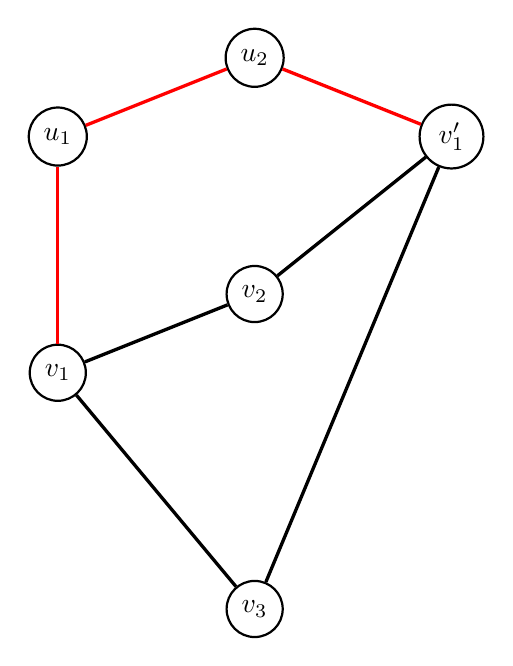
\begin{tikzpicture}
			\begin{scope}[every node/.style={circle,thick,draw}]
				\node (A) at (0,0) {$v_1$};
				\node (B) at (0,3) {$u_1$};
				\node (C) at (2.5,4) {$u_2$};
				\node (D) at (2.5,1) {$v_2$};
				\node (E) at (2.5,-3) {$v_3$};
				\node (F) at (5,3) {$v_1'$} ;
			\end{scope}
			\begin{scope}[>={[black]},
				every edge/.style={draw=red,very thick}]
				\path [->] (A) edge  (B);
				\path [->] (B) edge  (C);
				\path [->] (C) edge  (F);
			\end{scope}
			\begin{scope}[>={[black]},
				every edge/.style={draw=black,very thick}]
				\path [->] (A) edge  (D);
				\path [->] (A) edge  (E);
				\path [->] (D) edge  (F);
				\path [->] (E) edge  (F); 
			\end{scope}
		\end{tikzpicture}
	\end{figure}
	\newpage
	\textbf{Justification of Lemma \ref{lemma:3VerticeInOneCycle}:}

	Say we want to prove that there is a cycle containing vertices $a,b,c$. By fact one we know there is cycle containing $a,b$; a cycle containing $a,c$; and a cycle containing $b,c$. Merge this three cycles, we get a greater cycle containing $a,b,c$.

	

\end{solution}


\newpage

\begin{problem}{2}\textbf{[5pts]}
Let $S$ be a subset of edges of a \textbf{connected} graph $G$ which has an edge \textbf{(can have more than one!)} in common with every spanning \textbf{tree} of $G$.  Prove that $S$ contains a cutset of $G$.
\end{problem}
\begin{solution}
	Assuming that $S$ contains not a cutset, then $G \backslash S$ is a connected graph. We can construct a spanning tree from $G \backslash S$, that is a spanning tree of $G$ but contains no shared edge with $S$. This is a contradiction and we conclude that $S$ must contain a cutset.
\end{solution}

\end{document}
